% use command pdflatex filename.tex
\documentclass{article}
% \usepackage[noend]{algpseudocode}
% \usepackage{parskip}
% \usepackage{tikz, changepage, amssymb}
% \usetikzlibrary{automata,positioning,arrows}
\usepackage{amsmath, amsthm}
\usepackage{listings}
\usepackage{xcolor}
\usepackage{tikz}
\usepackage{array}
\usepackage{url, hyperref}
\usepackage{graphicx}
\graphicspath{{./images/}}


\lstset{
  language=python,
  basicstyle=\ttfamily,
  mathescape,
  morecomment=[l][\color{olive}]{\#},
  breaklines=true,
  postbreak=\space
}
\title{DATASCI 2G03 Project Report \\\large
Elastic Collisions between Contained Particles}
\author{Anthony Hunt}

\begin{document}
\maketitle

\section{Introduction}
Visualizing the effects of colliding elastic objects enables a clearer understanding of extremely small or extremely large natural phenomena,
especially in the fields of astrophysics (eg. rotation of stars in a galaxy) and chemistry (eg. ideal gas, electron/proton interactions).
Tools of this nature can provide intuition and a sense of familiarity to those studying these areas.
Even in everyday life, this type of simulation often appears in video games like pong, brick breaker, and 8 ball pool.
Therefore, this project attempts to simulate interactions between a large number of objects through
the motion and collision of moving particles.

The simplest of these interactions are those that do not involve a change in acceleration,
such as an ideal gas in a finite box. Wikipedia has an excellent example of one such simulation
\footnote{\url{https://en.wikipedia.org/wiki/Maxwell\%E2\%80\%93Boltzmann_distribution}}.
% \footnote{\url{https://en.wikipedia.org/wiki/Maxwell\%E2\%80\%93Boltzmann_distribution#/media/File:Simulation_of_gas_for_relaxation_demonstration.gif}}.
Further, a reasonable simulation should expect to converge to the Maxwell-Boltzmann distribution,
a chi-distribution with 3 degrees of freedom \footnote{\url{https://en.wikipedia.org/wiki/Chi_distribution}},
characterized by the large density of particles around the mean and the slow taper for higher particle speeds.

The first part of this project will consist of modelling the interaction between many particles
in a containing box the hopes of achieving a 2D Maxwell-Boltzmann distribution of velocities.
We also ensure correctness of our simulation by monitoring kinetic energy conservation for the system.
Then, we will extend these interactions with the addition of charged particles to simulate the effects of non-constant acceleration.
We do not expect the charged particles to follow the Maxwell-Boltzmann distribution,
but will explore other effects of remote particle-particle interactions, like orbits.


\section{Method}
\subsection{ODE Solver}
Since this simulation is based primarily around dynamic motion,
we will use the kick-drift-kick form of Leap Frog integration
\footnote{\url{https://en.wikipedia.org/wiki/Leapfrog_integration}}:
\begin{align}
    v_{i+\frac{1}{2}}&=v_{i}+a_{i}{\frac {\Delta t}{2}}\\
    x_{i+1}&=x_{i}+v_{i+\frac{1}{2}}\Delta t\\
    v_{i+1}&=v_{i+\frac{1}{2}}+a_{i+1}{\frac {\Delta t}{2}}
\end{align}

\subsection{Initial Equations}

The physics-based ODEs and other equations used to simulate this problem are listed below.
The goal of this simulation is to track the position of objects (represented by $x$)
over some length of time $t$. Each particle will have some mass $m$ and starting velocity $v$.

Velocity ($v$) of one particle
\footnote{\url{https://en.wikipedia.org/wiki/Equations_of_motion}}:
\begin{equation}
    v = \frac{dx}{dt}
\end{equation}

Acceleration ($a$) of one particle:
\begin{equation}
    a = \frac{dv}{dt} = \frac{d^2x}{dt^2}
\end{equation}

Kinetic energy of one particle:
\begin{equation}
E_k = \frac{1}{2}mv^2
\end{equation}

The below equation is used to calculate the vectors of velocity resulting from an elastic collision
\footnote{\url{https://en.wikipedia.org/wiki/Elastic_collision}}.
Let $v_1$ represent the first particle's velocity and $v_2$ for the second particle's velocity.
Additionally, let $v'$ represent the velocity after the collision and $v$ for the velocities prior to the collision.
Swapping $*_1$ and $*_2$ will provide the velocity for particle 2.

\begin{equation}
v'_1 = v_1 - \frac{2m_2}{m_1+m_2}\frac{\langle v_1 - v_2, x_1 - x_2 \rangle}{\|x_1-x_2\|^2}(x_1-x_2)
\end{equation}

\subsection{Extended Equations}

Newton's second law:
\begin{equation}
F = ma
\end{equation}

Coulomb's law: Force of charged particles against one another:
\begin{equation}
    F_{charge} = \frac{kq_1q_2}{r^2}
\end{equation}

Electric potential energy of a system
\footnote{\url{https://phys.libretexts.org/Bookshelves/University_Physics/University_Physics_(OpenStax)/University_Physics_II_-_Thermodynamics_Electricity_and_Magnetism_(OpenStax)/07\%3A_Electric_Potential/7.02\%3A_Electric_Potential_Energy}}:

\begin{equation}
    U = \frac{k}{2} \sum_i^N \sum_j^N \frac{q_iq_j}{r_{ij}} \text{for} i \neq j
\end{equation}

\subsection{Configuration Parameters}
\begin{itemize}
    \item Starting position $s$ of each particle
    \item Initial velocity $v$ of each particle
    \item Mass $m$ of each particle (kept at a constant 1 kg except for configuration 9)
    \item Radius of each particle $r$ (kept at a constant 0.25 m)
    \item Charge of different particles $q$ (kept at a constant $\pm 1$ except for configuration 9)
    \item Coulomb's constant $k$ (kept at $5 Nm^2/C$ instead of $9\times 10^9 Nm^2/C$ since we are massively downscaling real-world values)
\end{itemize}

\subsection{Interesting Properties}
\begin{itemize}
    \item Speed of particles over time (momentum of all particles should remain constant) position of particles on a graph
    \item Distribution of particle speeds (Maxwell-Boltzmann distribution)
    \item Unique path of each particle (random movement of one particle) \footnote{\url{https://en.wikipedia.org/wiki/Brownian_motion}}
\end{itemize}

\section{Testing}
To ensure the correctness of our program,
we compare the results of a few preset configurations against the expected behaviour of the simulation.
Additionally, we examine a collection of randomly positioned particles.

\subsection{Uncharged Particles}
The tests for this section cover the initial model of this project, without any extensions.
All particles are set to a charge of 0, so they only interact though collisions with other particles and walls.
This setup mimics that of an ideal gas, so we are expecting to find that energy is conserved and
the distribution of speed eventually forms the Maxwell-Boltzmann curve.

\subsubsection{2 Particles in a 1D Collision}
This test examines the effects of one collision between two particles moving towards one another on the x-axis,
as shown below. Both particles have the same initial speed and are pointed towards the origin:
\\
\begin{center}
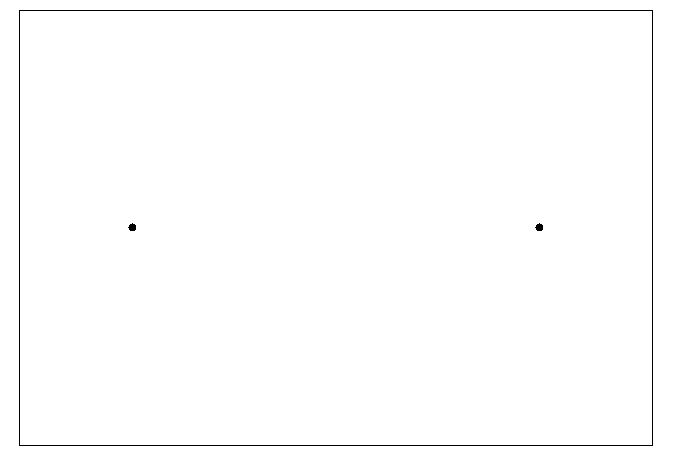
\includegraphics[scale=0.5]{uncharged_2_particles_1D}
\end{center}

Plotting the total energy and speed over time (blue and green respectively),
we find that kinetic energy is entirely conserved.
The purple line indicates electric potential energy and can be ignored.
Note that there is no scale for Time since this graph updates by combining new data every $dt$ seconds.
This means that initial iterations take up the entire plot and then compress as time goes on
and the plot holds more data.
\\
\begin{center}
    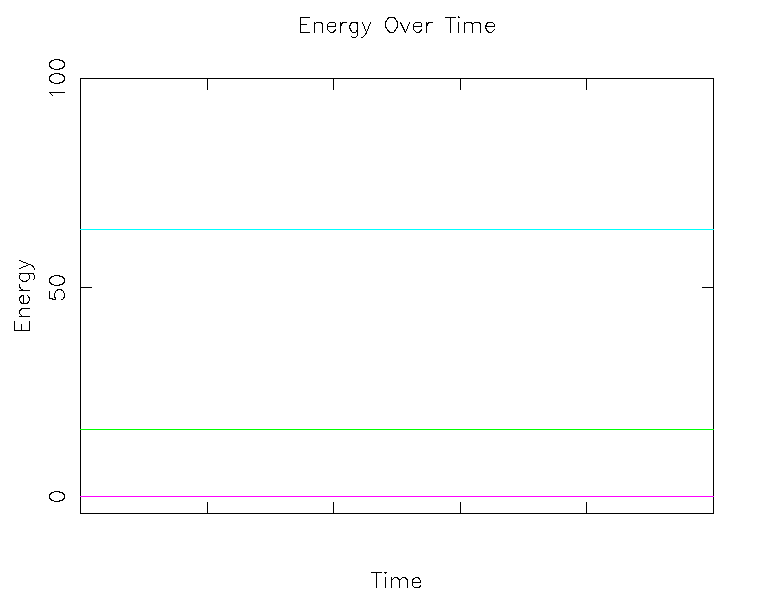
\includegraphics[scale=0.5]{uncharged_2_particles_1D_energy}
\end{center}

\subsubsection{2 Particles in an Angled Collision}
Similar to the previous test, but we now check that the angle of deflection for both particles are correct.
A simple case for examining angles is to move the point previously located at $(-1,0)$ to $(0,1)$ and point it towards the origin.
Thus, the two particles will meet at a 90-degree angle and bounce in perpendicular directions.
The initial layout of this test looks like (particles located at the top and right):
\\
\begin{center}
    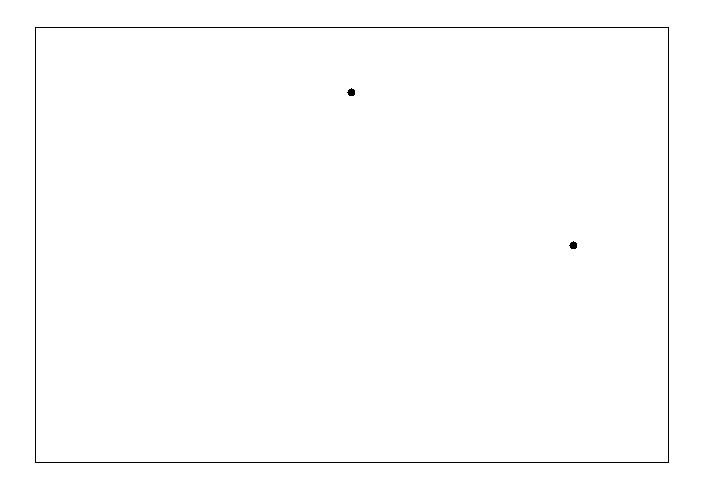
\includegraphics[scale=0.5]{uncharged_2_2D_start}
\end{center}

After collision, the initially top particle will be sent to the left and the right particle to the bottom.
Since the particles met at a 90-degree angle, they must depart at 90-degrees in order to conserve momentum
towards the bottom left.
\\
\begin{center}
    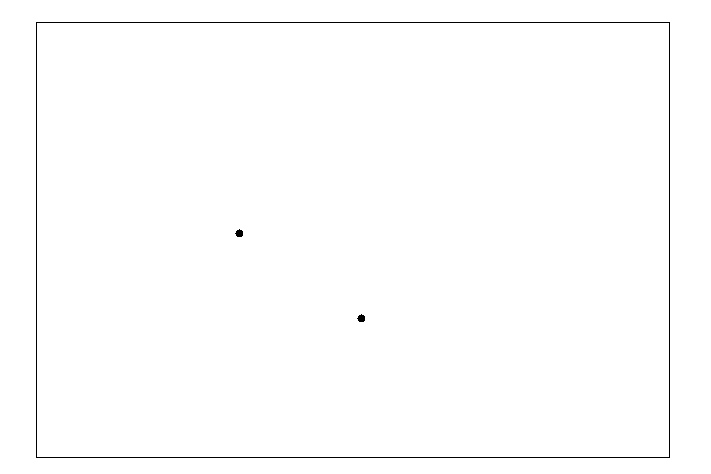
\includegraphics[scale=0.5]{uncharged_2_2D_after}
\end{center}

The particles will then bounce against the walls, reversing direction and colliding at the origin again.
Particle locations will swap between the two quadrants until the simulation is stopped.
Energy is conserved during this as both particles bounce with the same net speed
(although we do not include the energy vs time graph here since it looks the same as section 3.1.1).

\subsubsection{200 Random Particles}
With a large amount of particles, we can now examine the Maxwell-Boltzmann distribution.
The speed distribution of particles is separated into 30 ``buckets'',
where each bucket holds a range of particle speeds.
Note that the x-axis once again does not include precise velocity ranges,
since it is more important to visualize the groupings of particles rather than the exact speed of the particles themselves.

An image of the simulated particles is below:
\\
\begin{center}
    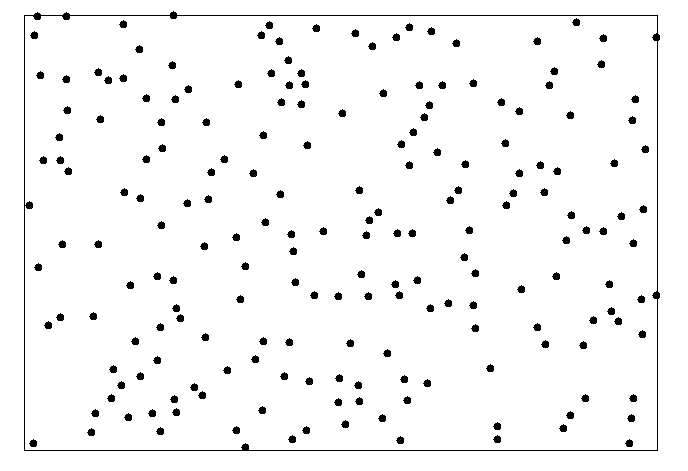
\includegraphics[scale=0.5]{uncharged_random}
\end{center}

After a few seconds of simulation, the distribution graph for 200 particles visibly relaxes from a random distribution
into the Maxwell-Boltzmann distribution.
\\
\begin{center}
    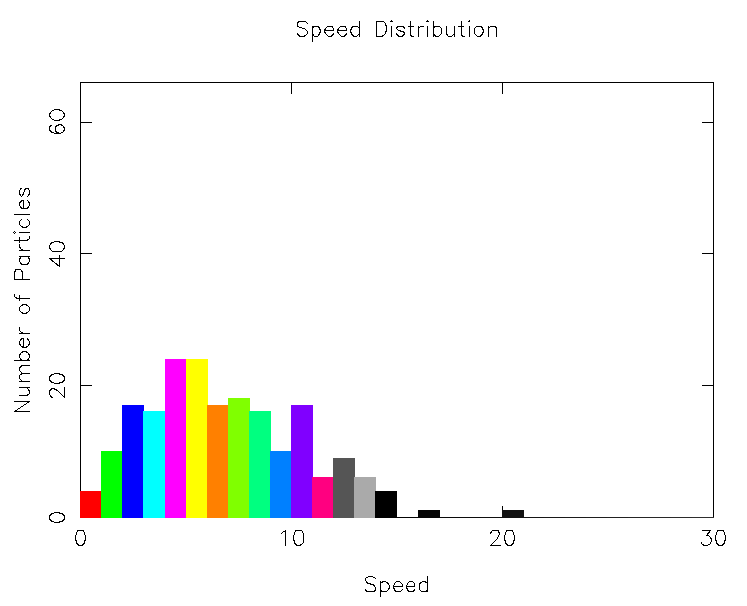
\includegraphics[scale=0.5]{uncharged_random_dist}
\end{center}

Calculating the exact curve of the distribution is slightly out of the scope of this project
since we do not have any information on gas-specific statistics (ie., temperature, pressure, heat),
but the characteristic bulge and slow taper can be visually estimated and compared with Wikipedia's simulation:
\\
\begin{center}
    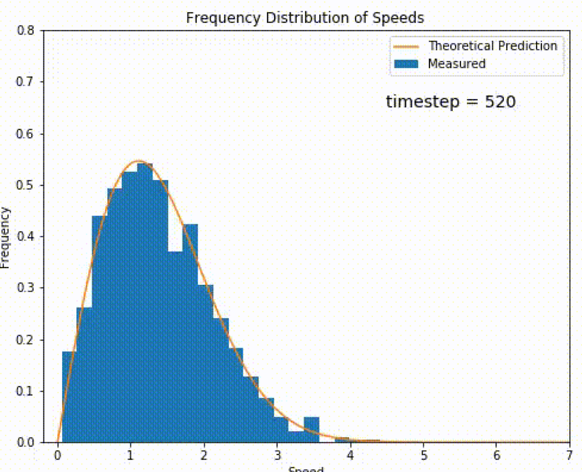
\includegraphics[scale=0.5]{mb_wiki}
\end{center}

Finally, we see that kinetic energy is indeed conserved, although total speed fluctuates within a margin of error.
\\
\begin{center}
    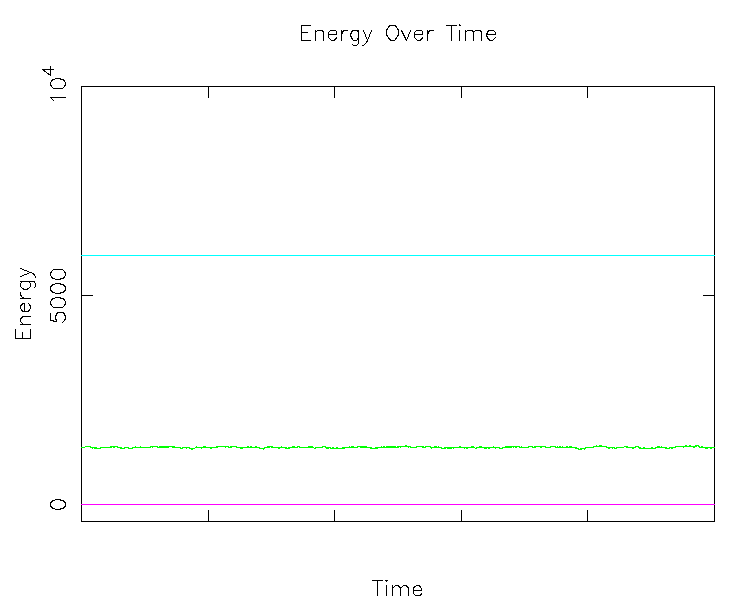
\includegraphics[scale=0.5]{uncharged_random_energy}
\end{center}

\subsection{Charged Particles}
The inclusion of charged particles within the simulation adds an additional ODE for our consideration,
namely, a non-constant acceleration due to Coulomb's Law.
The focus of this extension is to demonstrate how equations for dynamic particle movement
can be manipulated and reused to provide an idea of orbital movement.
Similar to gravity, the acceleration of charged particles is remotely influenced through other nearby particles.

\subsubsection{2 Particles in a 1D Collisions}
The same experiment for uncharged particles can be performed on charged particles.

For particles with the same charge, the setup is as follows (initial velocity towards the origin):
\\
\begin{center}
    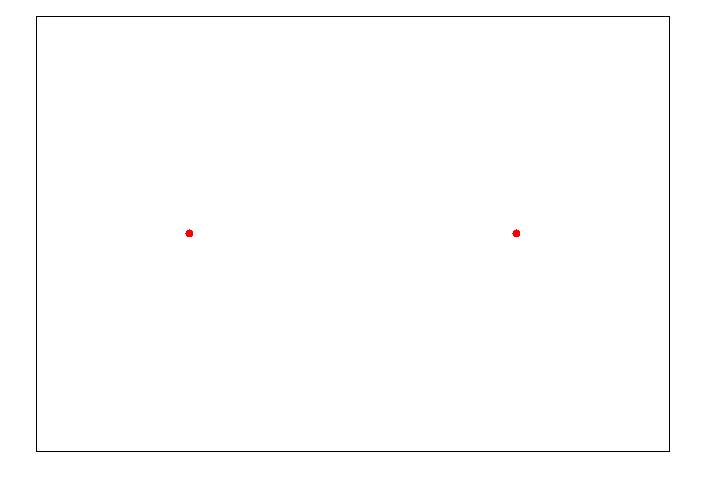
\includegraphics[scale=0.5]{charged_2_same}
\end{center}

As the particles approach one another, their speed and kinetic energy transform into electric potential energy.
Eventually, the particles stop a small distance before collisions and begin moving in the opposite direction.
Then, when moving apart, the potential energy is converted back into kinetic and the particles speed into the wall.
An oscillation pattern between the kinetic energy (blue) and electric potential (pink) can be seen below.
Interestingly, the total energy (black) appears to fluctuate due to time delays
converting between kinetic and electric energy.
The total energy has a slight monotonic change every iteration,
likely caused by the soft max function preventing particles from having
a distance smaller than some error value.
Although, these errors do not become obvious until after 5000 iterations of the simulation.
\\
\begin{center}
    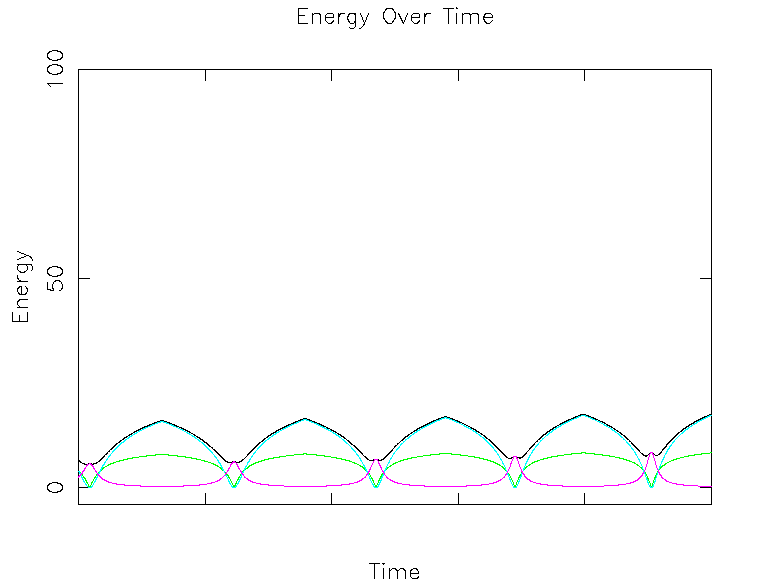
\includegraphics[scale=0.5]{charged_2_same_energy}
\end{center}

Similar behaviour can be seen for opposite charges, with the energy curves flipped:
\\
\begin{center}
    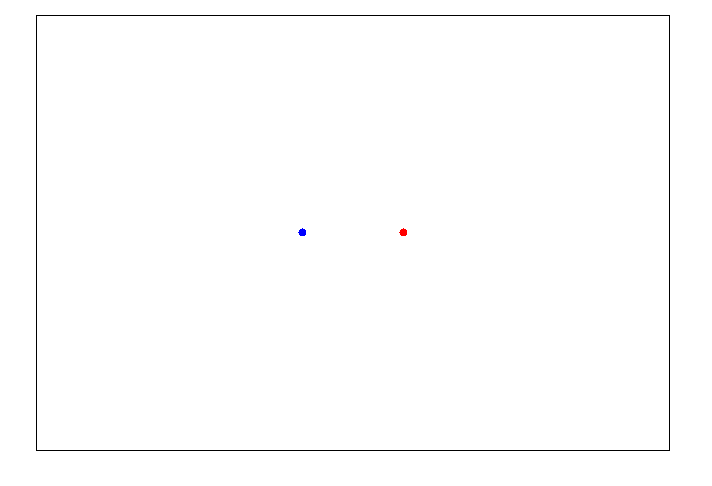
\includegraphics[scale=0.5]{charged_2_opp}
    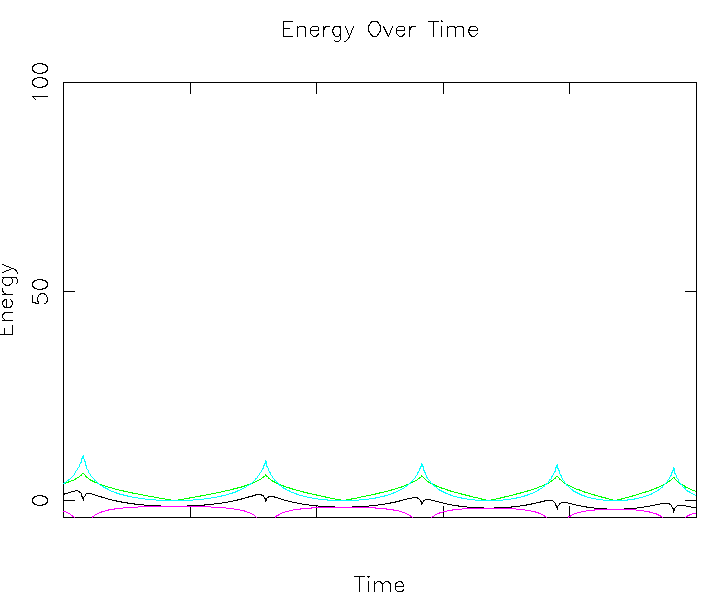
\includegraphics[scale=0.5]{charged_2_opp_energy}
\end{center}

In the case of particles attracted to one another, when collisions between particles were enabled,
the charged particles seemed to lose energy every iteration, slowing and eventually coming to a stop at the origin.
However, when collisions were disabled (so that particles had a radius of 0),
the system seemed to gain energy (shown below). Disabled collisions allowed
the particles to pass through one another (and the distance between them to become infinitesimally small) rather than colliding.0.
\\
\begin{center}
    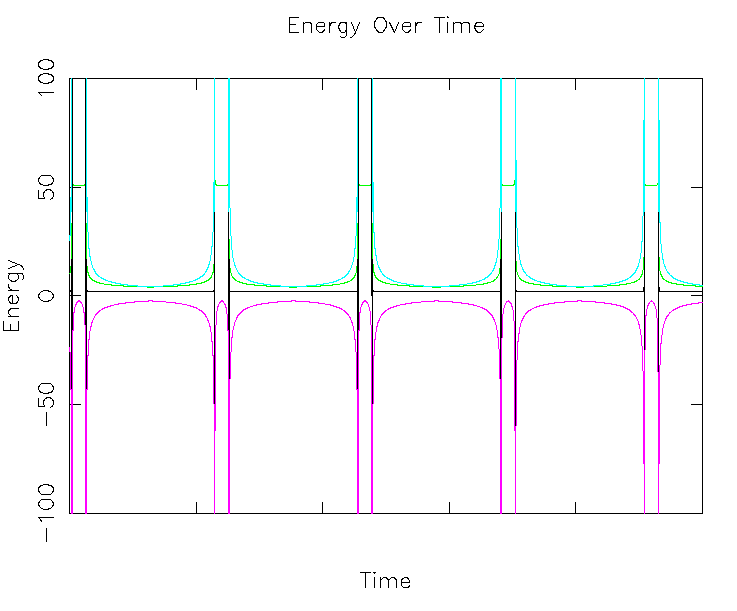
\includegraphics[scale=0.5]{charged_2_opp_energy_no_collision}
\end{center}

\subsubsection{Orbiting Particles}
Although the model may not perfectly conserve energy, we can still create simulations of orbits for a short period of time.
The below setup (with initial velocities pointed vertically and opposite to one another) led to a stable elliptical orbit about the origin.
\\
\begin{center}
    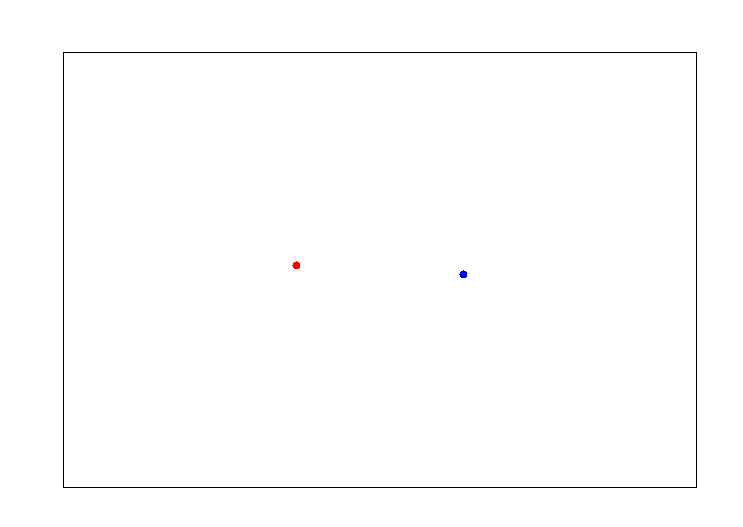
\includegraphics[scale=0.5]{orbit}
\end{center}

In the below graph, fluctuations in kinetic energy (blue) eventually stabilized into a consistent oscillation as well.
Note that electric potential energy (pink) is less than 0, so it does not display on the graph.
Instead, the effects of (the near-constant) electric potential can be seen through the total energy (black)
\\
\begin{center}
    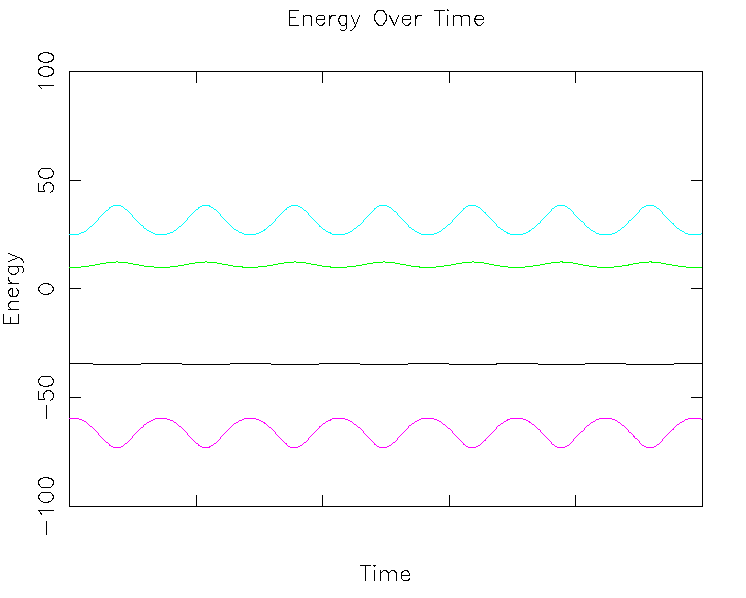
\includegraphics[scale=0.5]{orbit_energy}
\end{center}

Orbits akin to Bohr-Rutherford models of the atom,
where small charges orbit a large central charge,
can be seen by configuring several negatively charged masses initially travelling perpendicular to a large red mass, like below:
\\
\begin{center}
    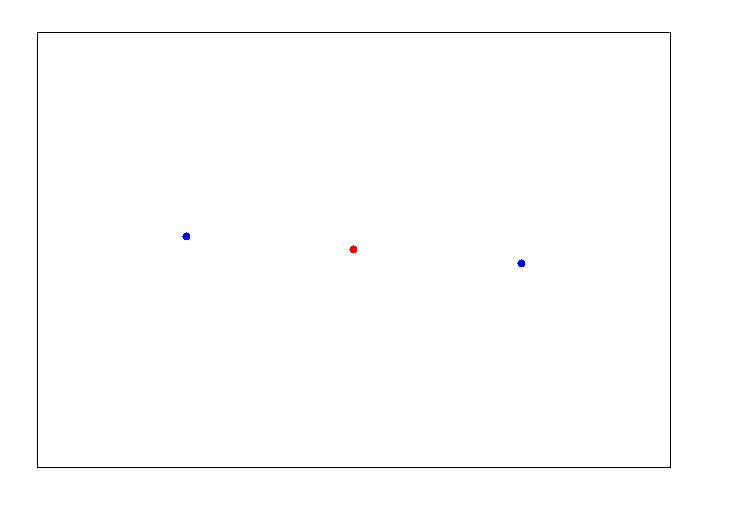
\includegraphics[scale=0.5]{atom}
\end{center}

\subsubsection{200 Random Particles}
This test is similar to that of the uncharged particles,
but all particles have been either assigned a positive (red) or negative (blue) charge.
The loss of energy conservation and differences between calculated electric potential energy
vs. kinetic energy are visible after $\approx 1000$ iterations of 200 randomly charged particles.
The setup and energy graphs are listed below:
\\
\begin{center}
    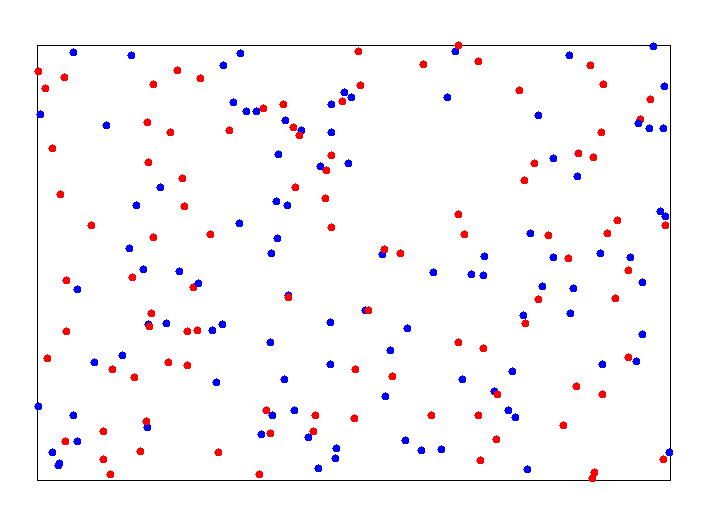
\includegraphics[scale=0.5]{charged_random}
    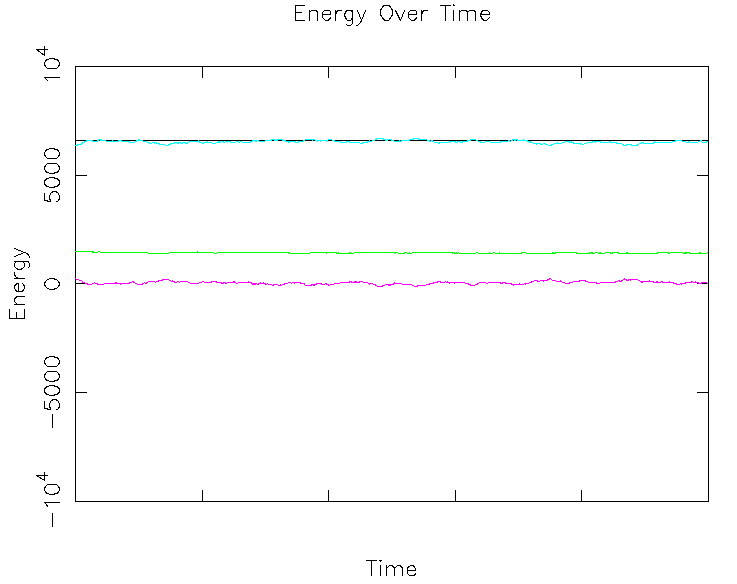
\includegraphics[scale=0.5]{charged_random_energy}
\end{center}

These random particles have a somewhat similar shape to the Maxwell-Boltzmann distribution, but with far more randomness.
In particular, buckets 12-20 contain far more particles than in section 3.1.3, and buckets 4-8 do not have a consistent sloped shape.
\\
\begin{center}
    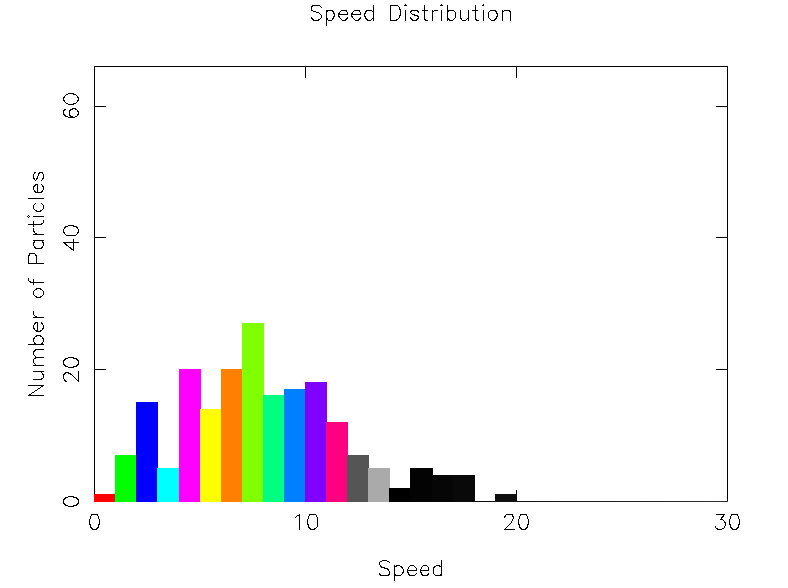
\includegraphics[scale=0.5]{charged_random_dist}
\end{center}


Note that for the above experiment, collisions were enabled.
Turning them off results in the following erratic graph, with large gains in total energy, similar results to section 3.2.1:
\\
\begin{center}
    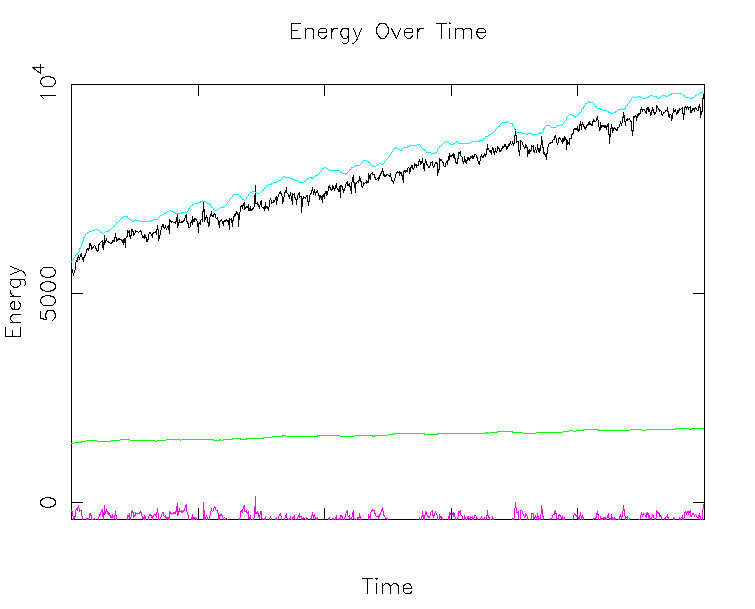
\includegraphics[scale=0.5]{charged_random_energy_no_collisions}
\end{center}


\section{Results}
The nature of this project and my simulation model is such that most interesting visuals
are the result of viewing updating graphs in real time.
Since snapshots of the model have been included as part of initial configuration for several tests above,
this section does not include any additional figures.
For consistency, this section only contains an analysis of the initial and extended tests described in section 3.

\subsection{Initial Model}
Overall, the basic model of uncharged particles behaved as expected
with respect to energy conservation and speed distribution.
Leap Frog integration had a high degree of precision for $>5000$ simulation iterations,
demonstrating its effectiveness for dynamic systems.

Initially, I faced difficulties with conservation of kinetic energy for uncharged particles
since some collisions would last for longer than one $dt$ instant.
To counter this, I implemented a directional check to ensure that particles only
collide when they are facing towards one another
\footnote{Dr. Wadsley initially told me about the equation, but the linked forum post also states the same method:
\url{https://math.stackexchange.com/questions/1438002/determine-if-objects-are-moving-towards-each-other}}.

Along with the above bug in collision calculations, I had also mistakenly tried calculating new velocities
based on the contributions of each particle at one point in time.
However, doing so led to very unpredictable behaviour when 3 or more particles collided at once.
Particles involved in complex collisions would either explode with speed or slow down immensely.
Eventually, this was resolved by calculating the pairwise collisions of every particle in some arbitrarily chosen order.

Although the energy-time graphs are not very interesting in section 3.1,
they serve as a constant, visual examination of the total energy of the system.
For a simulation with no explicit acceleration changes, all lines on the graph should appear as flat line.

\subsection{Extended Model}
Since charged particles were used with a mass of $1 kg$ and charges equal to $\pm 1 C$,
a far lower Coulomb constant $k$ was necessary to prevent extreme changes in acceleration.
Dealing with extreme values in the case of charged particles was especially difficult,
as floating point exceptions and segmentation faults often occurred as a result of
particles escaping the boundaries or coming in close contact with one another.

Enabling collisions during testing did produce some curious but reasonable results.
In the case of two oppositely-charged particles coming in contact,
the drop in net energy makes sense since both particles
would have felt a net acceleration almost always against the reversed velocities of any collisions,
slowly reducing the net speed of the system.
In other words, the initial potential energy could not entirely convert into kinetic energy
before the two particles collided. So when the velocity of each particle was reversed due to the collision equations,
the acceleration due to electric forces appeared to cause a loss in energy.
In the future, our simulation could attempt to counteract this loss
by temporarily disabling the acceleration at the point of collision,
but is beyond the scope of the project.
In reality, real-world charged particles are too small and too close together
to follow simplified collision rules based on rules of momentum and energy conservation.
Other laws take hold to dictate the flow of energy.

For tests with collisions disabled, as mentioned in section 3.2.1,
monotonic changes in the total system energy could be caused
by the soft max function limiting acceleration due to surrounding charges.

While the charged particle model massively simplifies all the complex interactions between particles in the real world,
the visualization of interacting particles is more than reasonable for at least the first 1000 iterations of $dt$,
before calculation errors cumulate.
With the charged model, we can plainly see physical phenomena like orbital movement as a product of a constant central acceleration
and an appropriate starting velocity.

\section{Future Work}
Both models performed well enough for the scope of this project,
but there is far more that could be done to explore this topic further:
\begin{itemize}
    \item Incorporation of gravity as an optional force.
    Implementing this with the current state of my project should not be terribly difficult,
    since a developer would only need to add the force of gravity to the collection of acceleration contributions.
    The two independent variables, mass and distance, are accessible within each particle's object.
    \item Expanding the container to a variety of different shapes.
    This would necessarily involve improvements to wall collision calculations in accommodating angles or curves.
    \item Improve wall bounce calculations to ensure that out-of-bounds objects are pushed back in bounds.
    Currently, if objects have enough velocity and acceleration away from the origin, the naive velocity reversal
    calculations of \texttt{Container::get\_collision\_velocity} may not be enough to keep it in bounds.
    \item Improve program efficiency from $O(n^2)$ to $O(n\log{n})$ by dividing the space
    and calculating collisions only for those objects close to one another.
    One of the more recent lectures have also explored an optimal
    method of calculating distant-dependent forces using a divide and conquer method.
    \item Add friction or an electric field map to provide non-constant acceleration outside of particle-particle interactions.
    This would enable the model to run other physics-based simulations like a mass spectrometer or even projectile motion
    (eg. a positively charged particle with a negatively charged bottom plate).
    \item Count the number of collisions between particles against a wall.
    3Blue1Brown has an excellent video exploring a special case where large
    masses collide with small masses with a ratio $\pi\times 10^x$ where $x$ is based on the ratio of the object masses
    \footnote{\url{https://www.youtube.com/watch?v=jsYwFizhncE}}.
    \item Examine the overall (conservation of) momentum of the system over time.
    \item Calculations for pressure, temperature, etc. in the context of the ideal gas law.
    This would also enable a direct overlay of the Maxwell-Boltzman distribution.
    \item Interactivity improvements, like adding energy to the system in the form of heat, controlling select particles,
    or tracing the path of selected particles to find random walk behaviour
    \footnote{\url{https://en.wikipedia.org/wiki/Brownian_motion}}.
\end{itemize}

\section{Conclusion}
Exploring and researching about particle simulation in the context of C++
helped me gain a deeper understanding and appreciation of physical interactions.
Among the most interesting findings was the mimicking of orbiting
objects through charged particles with select initial velocities,
the Maxwell-Boltzmann distribution of neutral particles,
and watching the randomness of an ideal gas particle's path.



\end{document}
